\documentclass[tikz,border=12pt]{standalone}
\usepackage[utf8]{inputenc}
\usepackage[T1]{fontenc}
\usepackage{lmodern}
\usepackage{amsmath}
\usetikzlibrary{arrows.meta,positioning,fit,backgrounds}

\definecolor{coseblue}{RGB}{0,70,140}
\definecolor{coseteal}{RGB}{22,138,128}
\definecolor{coseamber}{RGB}{217,119,6}
\definecolor{cosered}{RGB}{185,28,28}
\definecolor{slatebg}{RGB}{248,250,252}
\definecolor{slateborder}{RGB}{148,163,184}
\definecolor{slatetext}{RGB}{71,85,105}

\begin{document}
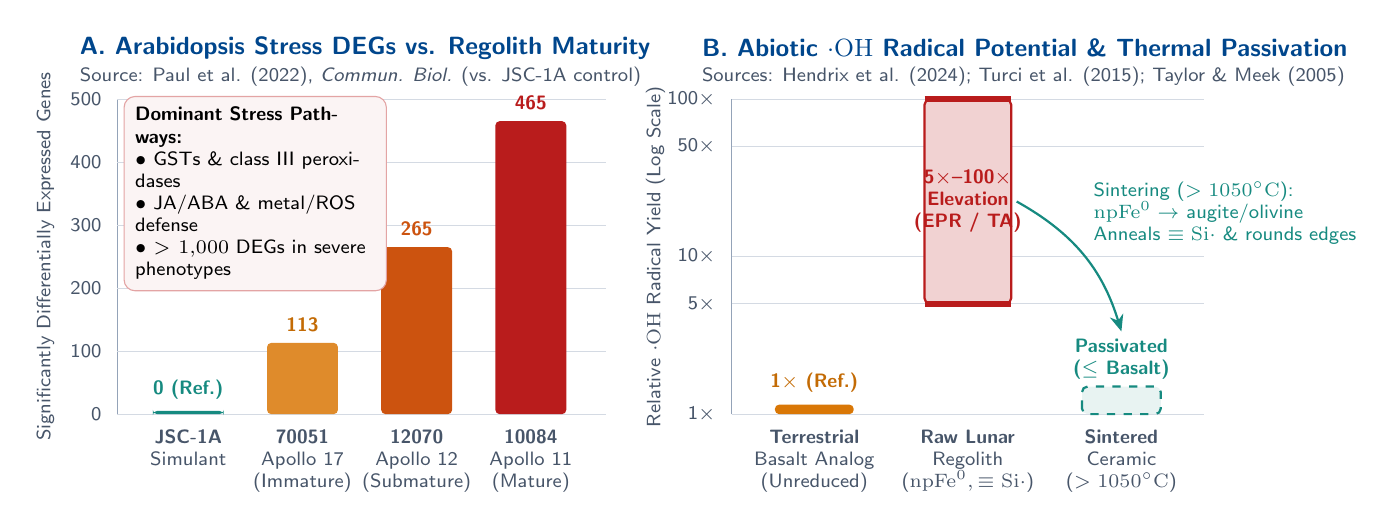
\begin{tikzpicture}[
    font=\sffamily\small,
    paneltitle/.style={
        font=\sffamily\bfseries\small,
        text=coseblue,
        anchor=west
    },
    axislabel/.style={
        font=\sffamily\scriptsize,
        text=slatetext
    },
    barlabel/.style={
        font=\sffamily\bfseries\scriptsize,
        anchor=south
    }
]

% =========================================================================
% PANEL A: PAUL ET AL. (2022) APOLLO REGOLITH DEGs
% =========================================================================
\node[paneltitle] at (-0.6, 5.15) {A. \textit{Arabidopsis} Stress DEGs vs. Regolith Maturity};
\node[axislabel, anchor=west] at (-0.6, 4.78) {Source: Paul et al. (2022), \textit{Commun. Biol.} (vs. JSC-1A control)};

% Axes for Panel A (x from 0 to 6.2, y from 0 to 4.2 -> 0 to 500 DEGs, scale: 100 DEGs = 0.8 cm)
\draw[slateborder, thin] (0, 0.5) -- (6.2, 0.5);
\draw[slateborder, thin] (0, 0.5) -- (0, 4.5);

% Y-axis grid & ticks (0, 100, 200, 300, 400, 500)
\foreach \val/\y in {0/0.5, 100/1.3, 200/2.1, 300/2.9, 400/3.7, 500/4.5} {
    \draw[slateborder!40, thin] (0, \y) -- (6.2, \y);
    \node[axislabel, anchor=east] at (-0.08, \y) {\val};
}
\node[axislabel, rotate=90, anchor=south] at (-0.68, 2.5) {Significantly Differentially Expressed Genes};

% Bars: JSC-1A (0), A17 70051 (113 -> 0.904 cm), A12 12070 (265 -> 2.12 cm), A11 10084 (465 -> 3.72 cm)
% Bar 1: JSC-1A
\fill[coseteal, rounded corners=1.5pt] (0.45, 0.5) rectangle (1.35, 0.54);
\node[barlabel, text=coseteal] at (0.90, 0.56) {0 (Ref.)};
\node[axislabel, align=center, anchor=north] at (0.90, 0.42) {\textbf{JSC-1A}\\Simulant};

% Bar 2: Apollo 17 (70051)
\fill[coseamber!85, rounded corners=1.5pt] (1.90, 0.5) rectangle (2.80, 1.404);
\node[barlabel, text=coseamber!90!black] at (2.35, 1.42) {113};
\node[axislabel, align=center, anchor=north] at (2.35, 0.42) {\textbf{70051}\\Apollo 17\\(Immature)};

% Bar 3: Apollo 12 (12070)
\fill[coseamber!60!cosered, rounded corners=1.5pt] (3.35, 0.5) rectangle (4.25, 2.62);
\node[barlabel, text=coseamber!60!cosered] at (3.80, 2.64) {265};
\node[axislabel, align=center, anchor=north] at (3.80, 0.42) {\textbf{12070}\\Apollo 12\\(Submature)};

% Bar 4: Apollo 11 (10084)
\fill[cosered, rounded corners=1.5pt] (4.80, 0.5) rectangle (5.70, 4.22);
\node[barlabel, text=cosered] at (5.25, 4.24) {465};
\node[axislabel, align=center, anchor=north] at (5.25, 0.42) {\textbf{10084}\\Apollo 11\\(Mature)};

% Callout inside Panel A
\node[draw=cosered!40, fill=cosered!5, rounded corners=4pt, inner sep=4pt, font=\sffamily\scriptsize, align=left, text width=3.05cm] at (1.75, 3.30) {
    \textbf{Dominant Stress Pathways:}\\
    $\bullet$ GSTs \& class III peroxidases\\
    $\bullet$ JA/ABA \& metal/ROS defense\\
    $\bullet$ $>1{,}000$ DEGs in severe phenotypes
};

% =========================================================================
% PANEL B: ABIOTIC OH RADICAL ELEVATION & SINTERING PASSIVATION
% =========================================================================
\begin{scope}[shift={(7.8, 0)}]
\node[paneltitle] at (-0.5, 5.15) {B. Abiotic $\cdot\mathrm{OH}$ Radical Potential \& Thermal Passivation};
\node[axislabel, anchor=west] at (-0.5, 4.78) {Sources: Hendrix et al. (2024); Turci et al. (2015); Taylor \& Meek (2005)};

% Axes for Panel B (log10 scale from 0.5x to 150x -> y=0.5 is 1x, y=2.5 is 10x, y=4.5 is 100x)
\draw[slateborder, thin] (0, 0.5) -- (6.0, 0.5);
\draw[slateborder, thin] (0, 0.5) -- (0, 4.5);

% Y-axis log ticks: 1x (0.5), 5x (1.90), 10x (2.5), 50x (3.90), 100x (4.5)
\foreach \val/\y in {1$\times$/0.5, 5$\times$/1.90, 10$\times$/2.5, 50$\times$/3.90, 100$\times$/4.5} {
    \draw[slateborder!40, thin] (0, \y) -- (6.0, \y);
    \node[axislabel, anchor=east] at (-0.08, \y) {\val};
}
\node[axislabel, rotate=90, anchor=south] at (-0.72, 2.5) {Relative $\cdot\mathrm{OH}$ Radical Yield (Log Scale)};

% Column 1: Terrestrial Basalt (1x)
\fill[coseamber, rounded corners=1.5pt] (0.55, 0.5) rectangle (1.55, 0.62);
\node[barlabel, text=coseamber!90!black] at (1.05, 0.65) {1$\times$ (Ref.)};
\node[axislabel, align=center, anchor=north] at (1.05, 0.42) {\textbf{Terrestrial}\\Basalt Analog\\(Unreduced)};

% Column 2: Reduced Lunar Regolith / Simulant (5x - 100x range bar)
\fill[cosered!20, draw=cosered, thick, rounded corners=2pt] (2.45, 1.90) rectangle (3.55, 4.50);
\draw[cosered, line width=2pt] (2.45, 1.90) -- (3.55, 1.90);
\draw[cosered, line width=2pt] (2.45, 4.50) -- (3.55, 4.50);
\node[font=\sffamily\bfseries\scriptsize, text=cosered, align=center] at (3.00, 3.20) {5$\times$--100$\times$\\Elevation\\(EPR / TA)};
\node[axislabel, align=center, anchor=north] at (3.00, 0.42) {\textbf{Raw Lunar}\\Regolith\\($\mathrm{npFe}^0, \equiv\mathrm{Si}\cdot$)};

% Column 3: Sintered Ceramic (>1050 C Passivated)
\draw[coseteal, thick, dashed, fill=coseteal!10, rounded corners=2pt] (4.45, 0.5) rectangle (5.45, 0.85);
\node[font=\sffamily\bfseries\scriptsize, text=coseteal, align=center] at (4.95, 1.20) {Passivated\\($\le$ Basalt)};
\node[axislabel, align=center, anchor=north] at (4.95, 0.42) {\textbf{Sintered}\\Ceramic\\($>1050^\circ\mathrm{C}$)};

% Passivation arrow from Raw to Sintered
\draw[-{Stealth[length=6pt,width=5pt]}, thick, coseteal] (3.62, 3.20) to[bend left=22] node[midway, above right, font=\sffamily\scriptsize, text=coseteal, align=left] {Sintering ($>1050^\circ\mathrm{C}$):\\$\mathrm{npFe}^0 \to$ augite/olivine\\Anneals $\equiv\mathrm{Si}\cdot$ \& rounds edges} (4.95, 1.55);

\end{scope}

\end{tikzpicture}
\end{document}
